% !TEX root = ./rep.tex
\section{Demonstration Simulations}
\label{s:demo}

We demonstrate here the use of cardinal on two pebble-bed setups representative of FHR cores.

\subsection{146 Pebbles}
\label{ss:c4}

Using the Nek5000 model of the TAMU experiment as a basis, we have developed a multiphysics simulation of a bed comprising 146 pebbles.
The pebble model for Nek5000 reflects the practices used for the TAMU experiment, which were validated carefully against experimental PIV data. Inlet/outlet boundary conditions are used (Figure~\ref{f:pb2}). Unlike the TAMU experiment, here, the mesh is designed to allow clearance between pebbles. This facilitates the coupling, but it will likely be updated in future simulations. The difference is outlined in Figure~\ref{f:pb2}. The mesh comprises approximately roughly 500,000 elements overall, and it is designed to run at $N=5$ for coarse results and $N=7$ for finer simulations (for a max of 256 million grid points). We assume constant properties.

\begin{figure}[!h]
\centering
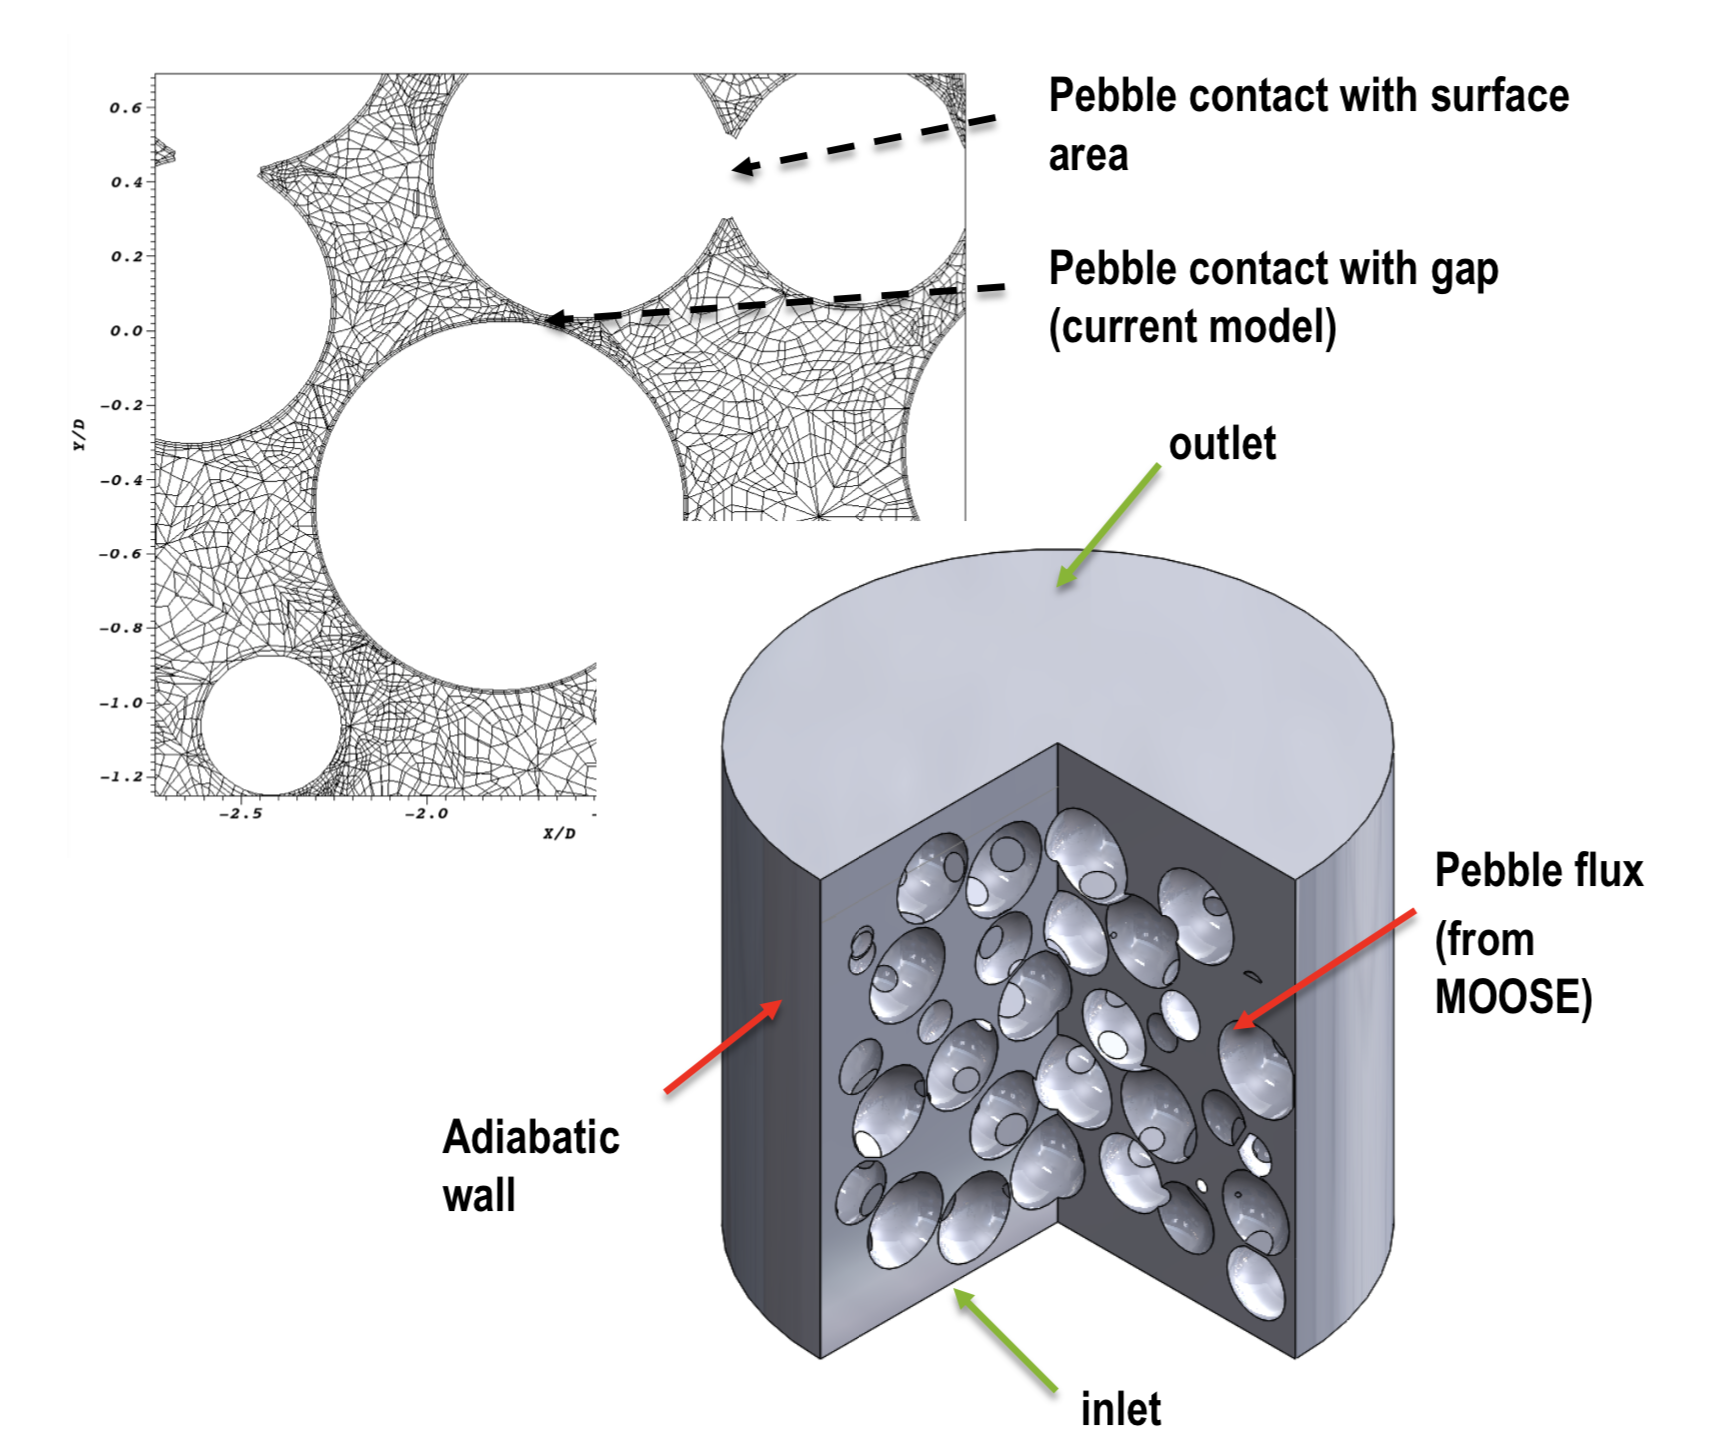
\includegraphics[clip=true,width=0.8\textwidth]{Figures/pb_mesh}
\caption{Mesh and boundary conditions for Nek5000 problem.}
\label{f:pb2}
\end{figure}

To test various options and accelerate the development, we defined four variants of the demo problem, all available in the Cardinal repository. The variants reflect the need to define cheaper transients for testing purposes. Table~\ref{tab:nek} shows the cases: they are listed in order of increasing computational cost. Restarting from an advanced restart leads to faster convergence. Moreover, simulating the full Navier-Stokes is considerably more expensive than assuming a ``frozen velocity'' and solving only the advection-diffusion equation.

\begin{table}
  \centering
  \begin{tabular}{|lcc|}
    \hline \hline
    Case & Restart condition & Solver \\
    \hline
    1 & Advanced restart state & Advection-Diffusion only \\
    2 & Constant temperature   & Advection-Diffusion only \\
    3 & Advanced restart state & Full Navier-Stokes \\
    4 & Constant temperature   & Full Navier-Stokes \\
    \hline \hline
  \end{tabular}
  \caption{Nek5000 cases with various solver options.}
  \label{tab:nek}
\end{table}

The OpenMC model is consistent with the pebble bed model discussed in the validation section. For BISON and the demonstration problem under consideration, we consider only the conduction equation, and as such, it is a relatively straightforward setup. Properties are constant and adapted from available correlations. The mesh for a single sphere is generated and replicated at run time. Only cell-based tallies are considered for this demonstration.

For the coupled simulations, we opt to tightly couple Nek5000 and BISON, and loosely couple OpenMC, given that if OpenMC is executed at every step, the computational cost becomes excessive. We perform the OpenMC solve every 100 steps. The simulations are performed on 2000 processors. Snapshots of the state after an initial transient are shown in Figure~\ref{f:dtamu1} and Figure~\ref{f:dtamu2}. In particular, we observe:
\begin{itemize}
  \item The effect of the complex flow field on the surface temperature of the pebbles.
  \item A slight tilt in the temperature distribution in the fuel's interior due to the outer temperature condition of each pebble.
  \item The effect of the reflective boundary conditions on the power distribution and a slight power tilt toward the bottom due to the colder coolant.
\end{itemize}

\begin{figure}[!h]
\centering
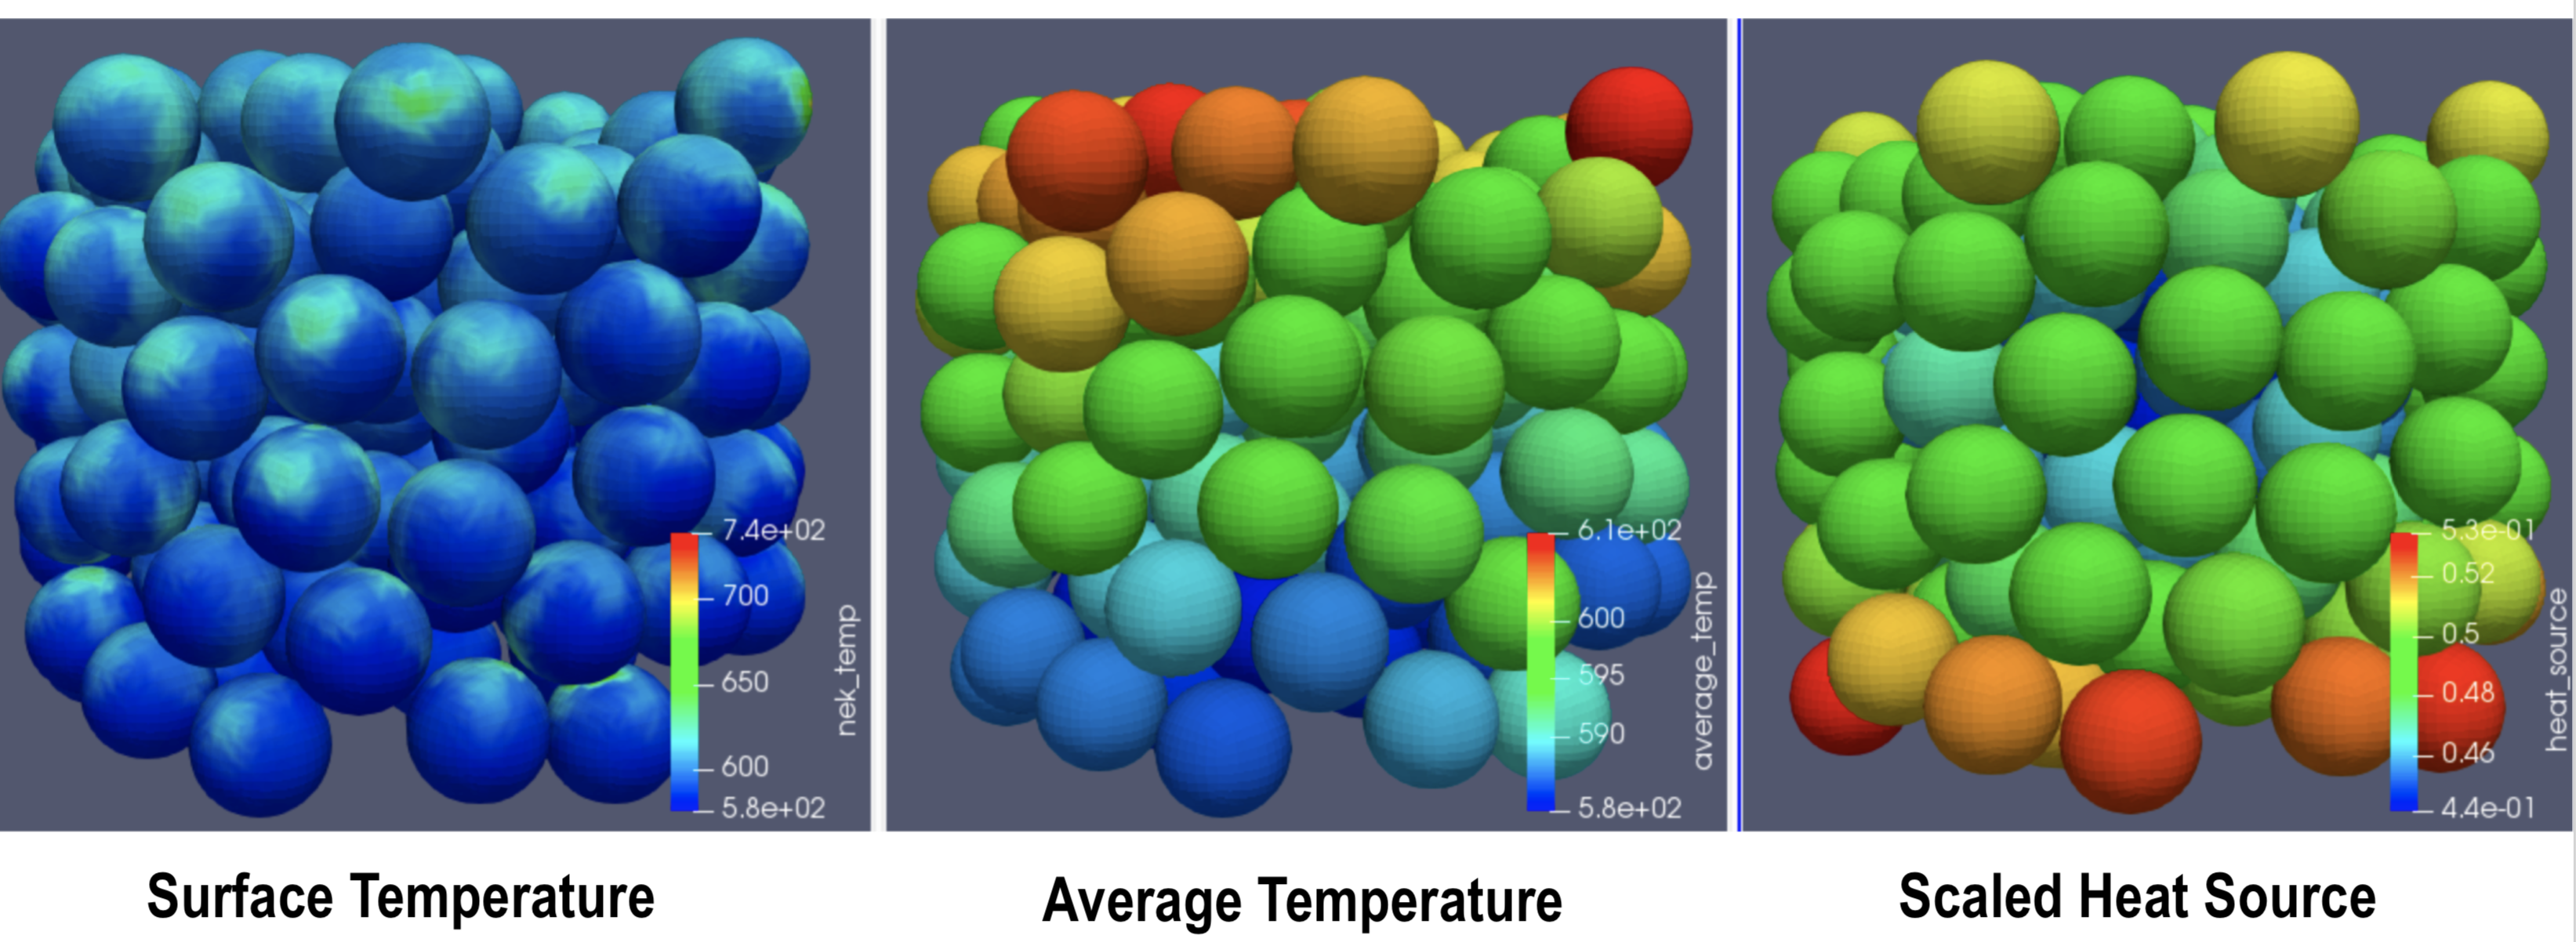
\includegraphics[clip=true,width=0.9\textwidth]{Figures/demo_r1}
\caption{TAMU demo Results. From left to right: snapshots of temperature on surface, average temperature in solid and average heating}
\label{f:dtamu1}
\end{figure}

\begin{figure}[!h]
\centering
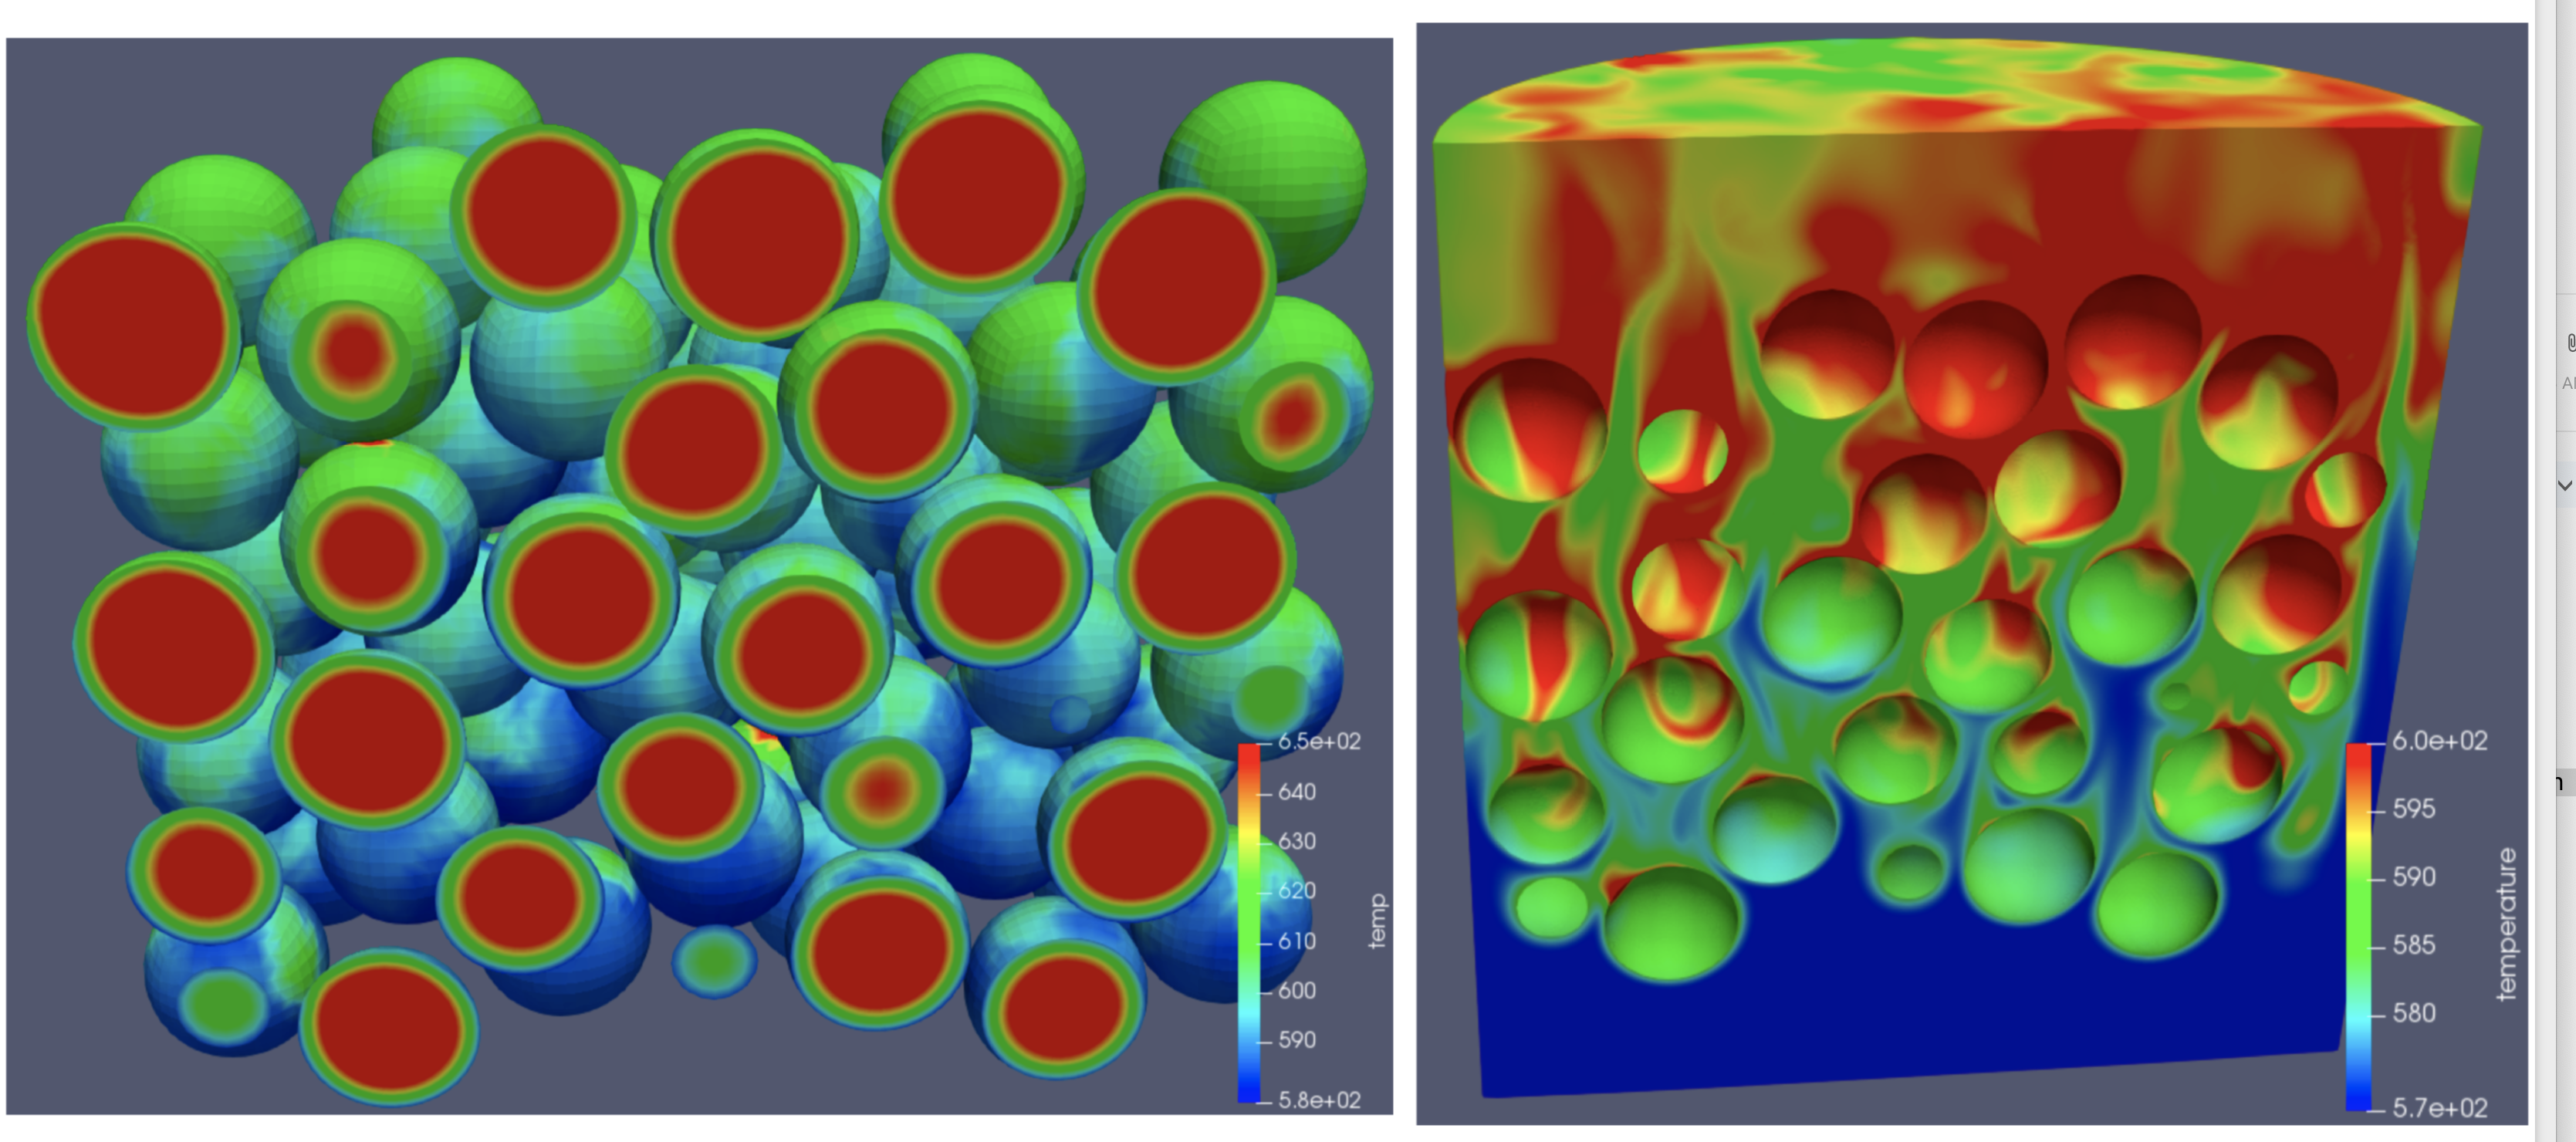
\includegraphics[clip=true,width=0.9\textwidth]{Figures/demo_r2}
\caption{TAMU Demo Results. Right - temperature in the solid. Left - temperature details in the fluid.}
\label{f:dtamu2}
\end{figure}

\subsection{1568 Pebbles}

\subsubsection{Numerical Setup}

We also present a case comprising 1568 pebbles. The pebble configuration has
been obtained using a discrete element method (DEM) code~\cite{projectChronoWebSite}.
A major overhaul on the mesh generation for the fluid domain was necessary
to automate as much as possible the process and to reduce the number of elements
per pebble. Our newly developed all-hex meshing tool, based on a Voronoi cell strategy,
allows us to produce high-quality hexahedral meshes using roughly 300--400 elements per pebble,
which gives a significant reduction in the element counts.

An example is provided in Figure~\ref{f:ndemo1}, for the 1568
pebble configuration. Higher pebble counts have a similar mesh density.
We note that 1568 pebbles is a significant size for a coupled calculation and
representative of the SANA experiments \cite{zou2017validation}, for instance.

\begin{figure}[!h]
\centering
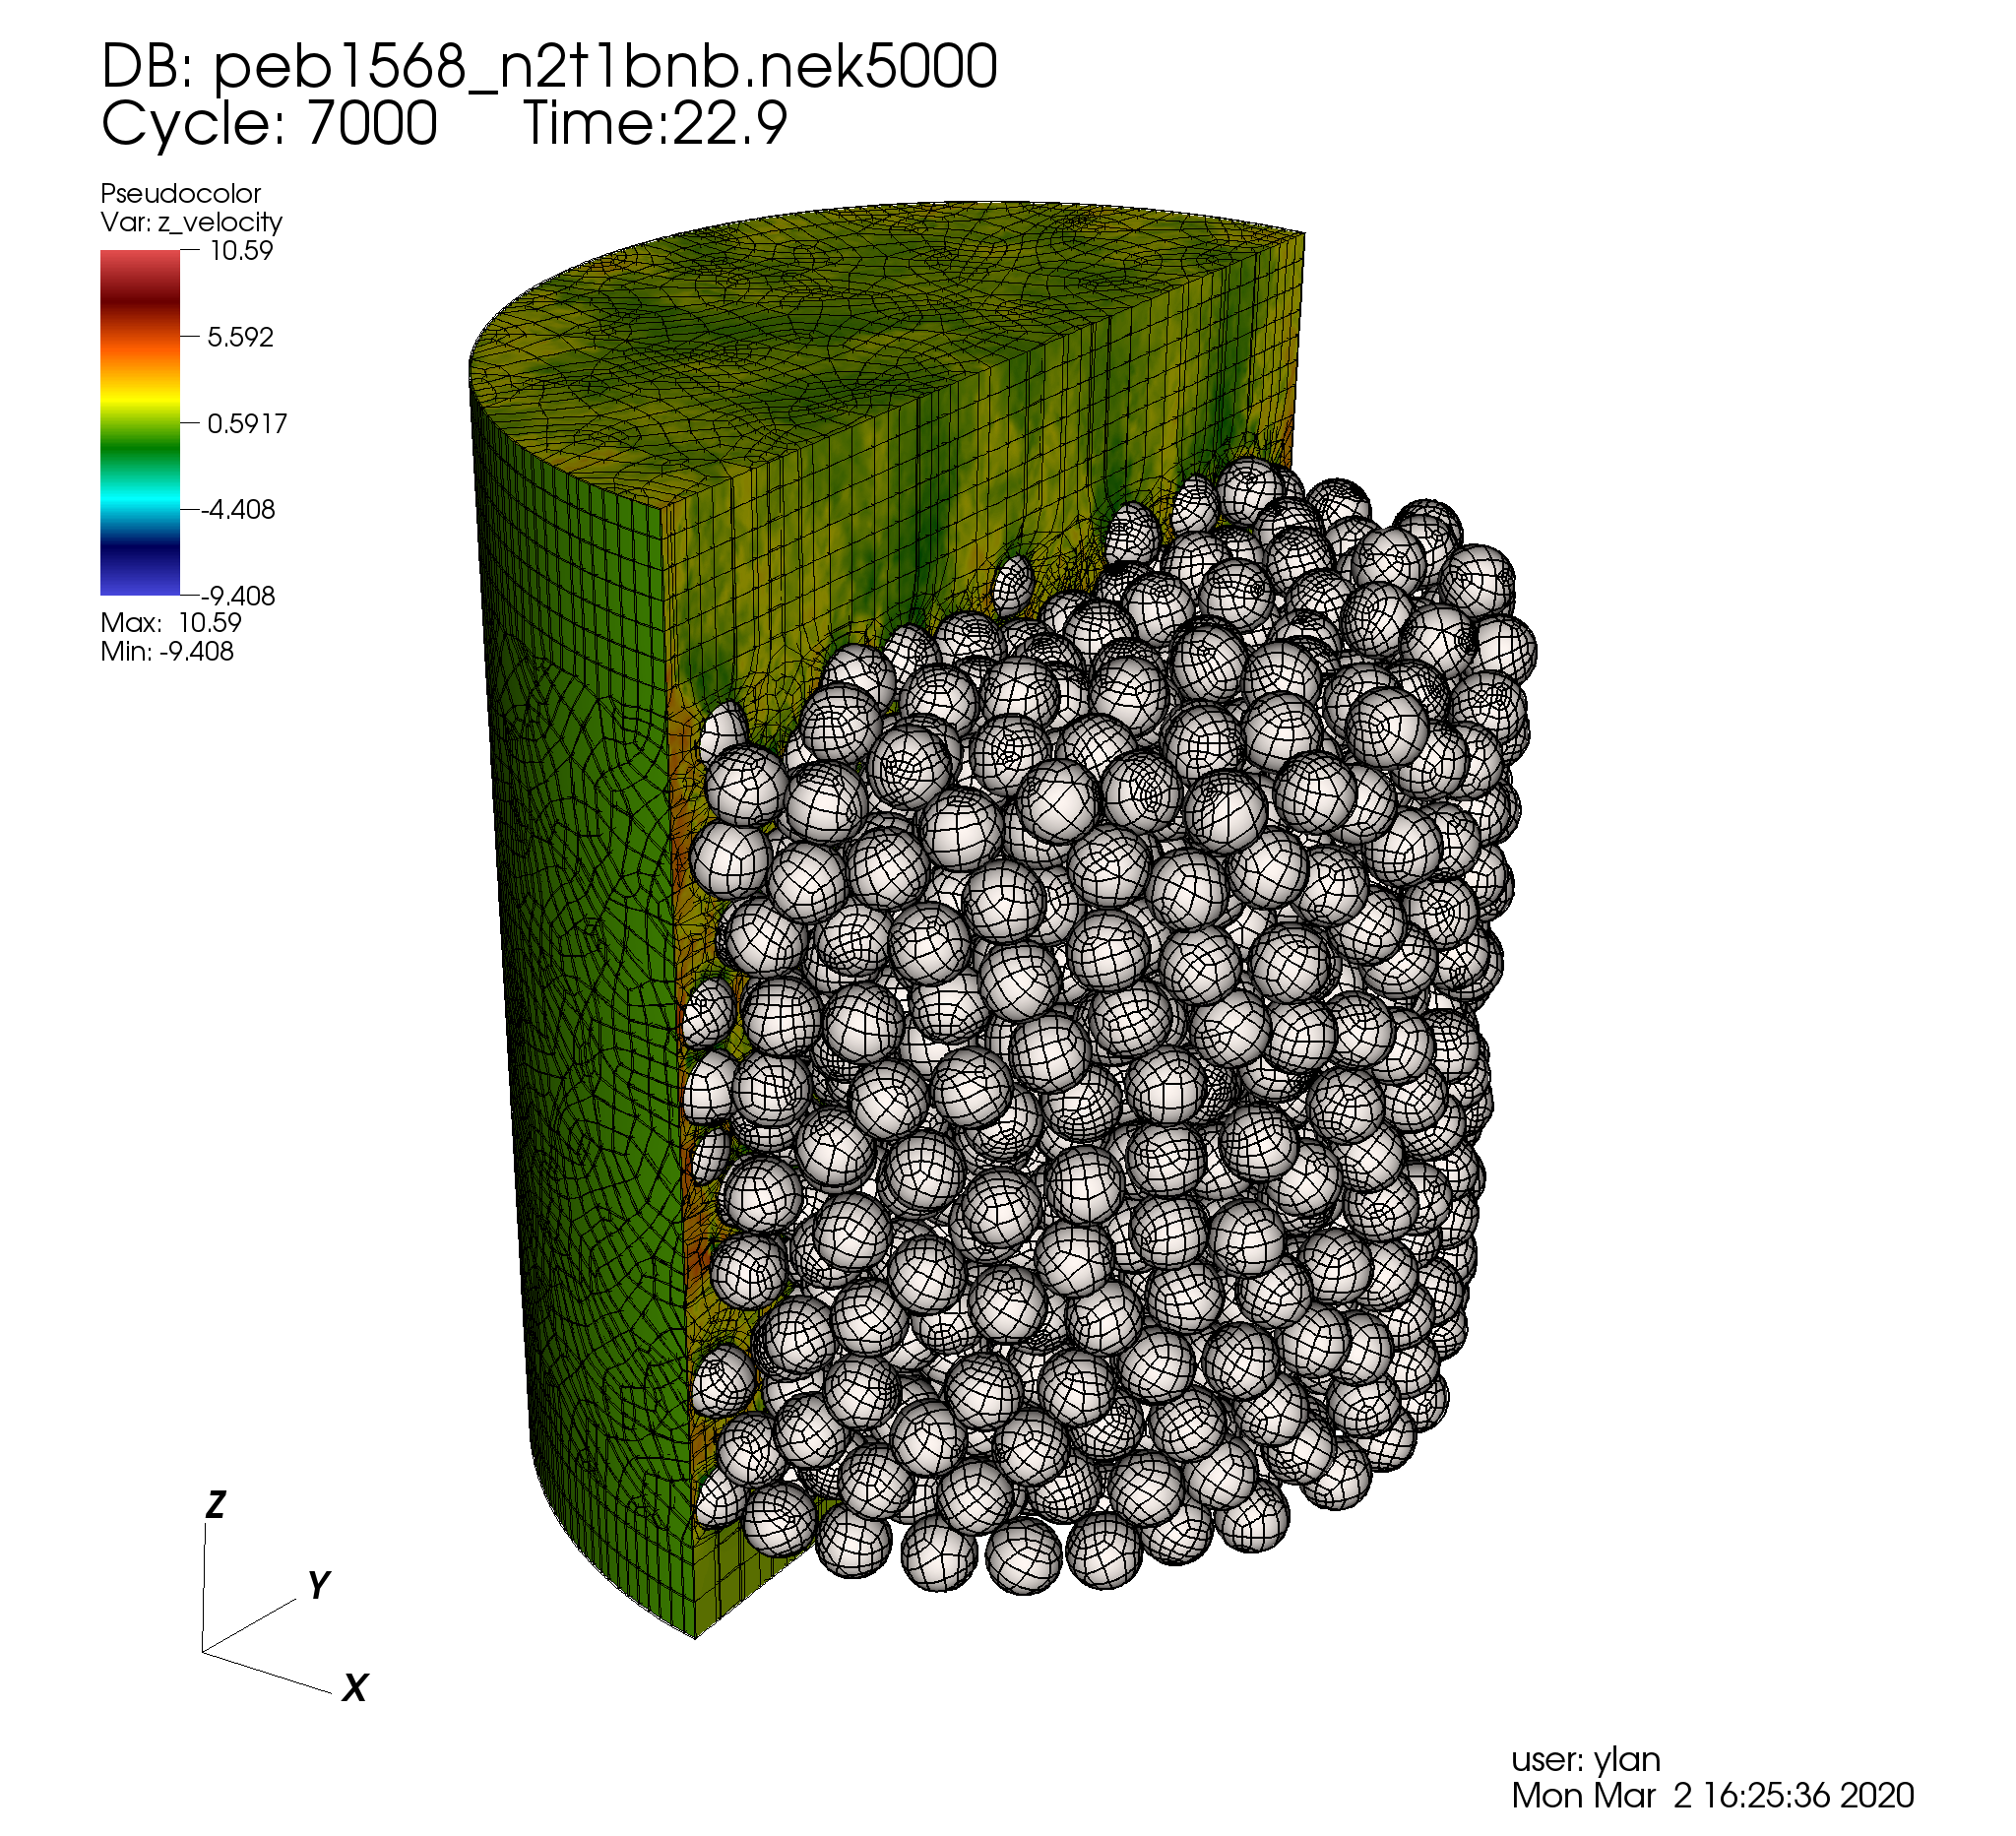
\includegraphics[clip=true,width=0.9\textwidth]{Figures/ndemo_r1}
\caption{NekRS: A spectral element mesh using 524,386 spectral elements for 1568 pebble configuration.
         The mesh is generated by all-hex meshing tool based on Voronoi cell strategy.}
\label{f:ndemo1}
\end{figure}

For this demonstration, the sizes and composition of the TRISO particles were based on TRISO manufactured at INL, following the practice established in the validation section. Though these particles were developed for the Advanced Gas Reactor (AGR) fuel, particles with the same specifications are used for FHR test reactors and computation benchmarks. The sizes and compositions of the pebbles were taken from the Mark-1 FHR reactor constructed at UC Berkeley. For BISON and the demonstration problem under consideration, we consider only the conduction equation, and as such, it is a relatively straightforward setup. Properties are constant and adapted from available correlations. The mesh for a single sphere is generated and replicated at run time. The same mesh is used for the mesh tallies in OpenMC.

\subsubsection{Results}
We begin with demonstrating strong-scaling performance of NekRS (GPU) and NekRS (CPU) in Table~\ref{tab:nekrs}.
We measure timings for 100 time steps for turbulent flow simulations with 1568-pebble mesh on ORNL’s Summit, 
using 42 MPI ranks per node for CPU runs and 6 Nvidia V100s per node for GPU runs. 
For the same node count, the GPU-accelerated variant of NekRS is more than 9$\times$ faster, when using
3.5 million points per GPU with 7283 spectral elements per GPU and $N=7$. 
NekRS GPU run realizes 82\% efficiency at 2.1 million points per GPU.


\begin{table}
  \centering
  \begin{tabular}{c|ccc||ccc}
    \hline \hline
 % \multirow{2}{*}{ } &
  \multicolumn{1}{c|}{ } &
  \multicolumn{3}{|c||}{NekRS GPU}  &
  \multicolumn{3}{|c}{NekRS CPU} \\
  \hline
  \hline
  %\cline{2-5}
    nodes  &  $E$ per GPU & time per step (sec) & efficiency & E per MPI& time per step (sec) & efficiency \\
  \hline
    12 & 7283 & 0.569 & 1.00 & 1040 & 5.361  & 1.00\\
    20 & 4369 & 0.416 & 0.82 & 624 & 3.055  & 1.05\\
    28 & 3121 & 0.338 & 0.72 & 445 & 2.200  & 1.04\\
    36 & 2427 & 0.309 & 0.61 & 346 & 1.876  & 0.95\\
    44 & 1986 & 0.290 & 0.53 & 283 & 1.401  & 1.04\\
    52 & 1680 & 0.255 & 0.51 & 240 & 1.204  & 1.02\\
    \hline \hline
  \end{tabular}
  \caption{NekRS GPU/CPU strong-scale timings (seconds per step) for 100 steps of turbulent flow simulations
   with $Re=10000$ for 1568-pebble case using total number of grid point $n=179,864,398$.}
  \label{tab:nekrs}
\end{table}

The model described in the previous section has been run on 12 and 20 nodes of Summit, with 6 MPI ranks on each node, corresponding to the 6 GPUs on each node. The OpenMC and BISON models are designed to run on CPU while the NekRS model runs on the GPU. Stand-alone NekRS simulations have been run first up to 25 convective time units to develop turbulence, which are shown in igure~\ref{f:ndemo3} using an LES approach.

A restart file has then been generated and used to restart a transient simulation in Cardinal representing the pebbles' heat-up. The time step has been fixed to $5\times 10^{-4}$ s in both BISON and NekRS. The temperature at time zero has been set to 300 $^{\circ}$C everywhere. Figure~\ref{f:ndemo4} presents the temperature at the surface of the pebbles in BISON at three points in time. The simulations took 2.5 s per coupled time step on 20 nodes, requiring transfer between physics at each timestep. However, this could be significantly optimized by relaxing the requirement, as data transfer from GPU to CPU should be minimized as much as possible.

\begin{figure}[!h]
\centering
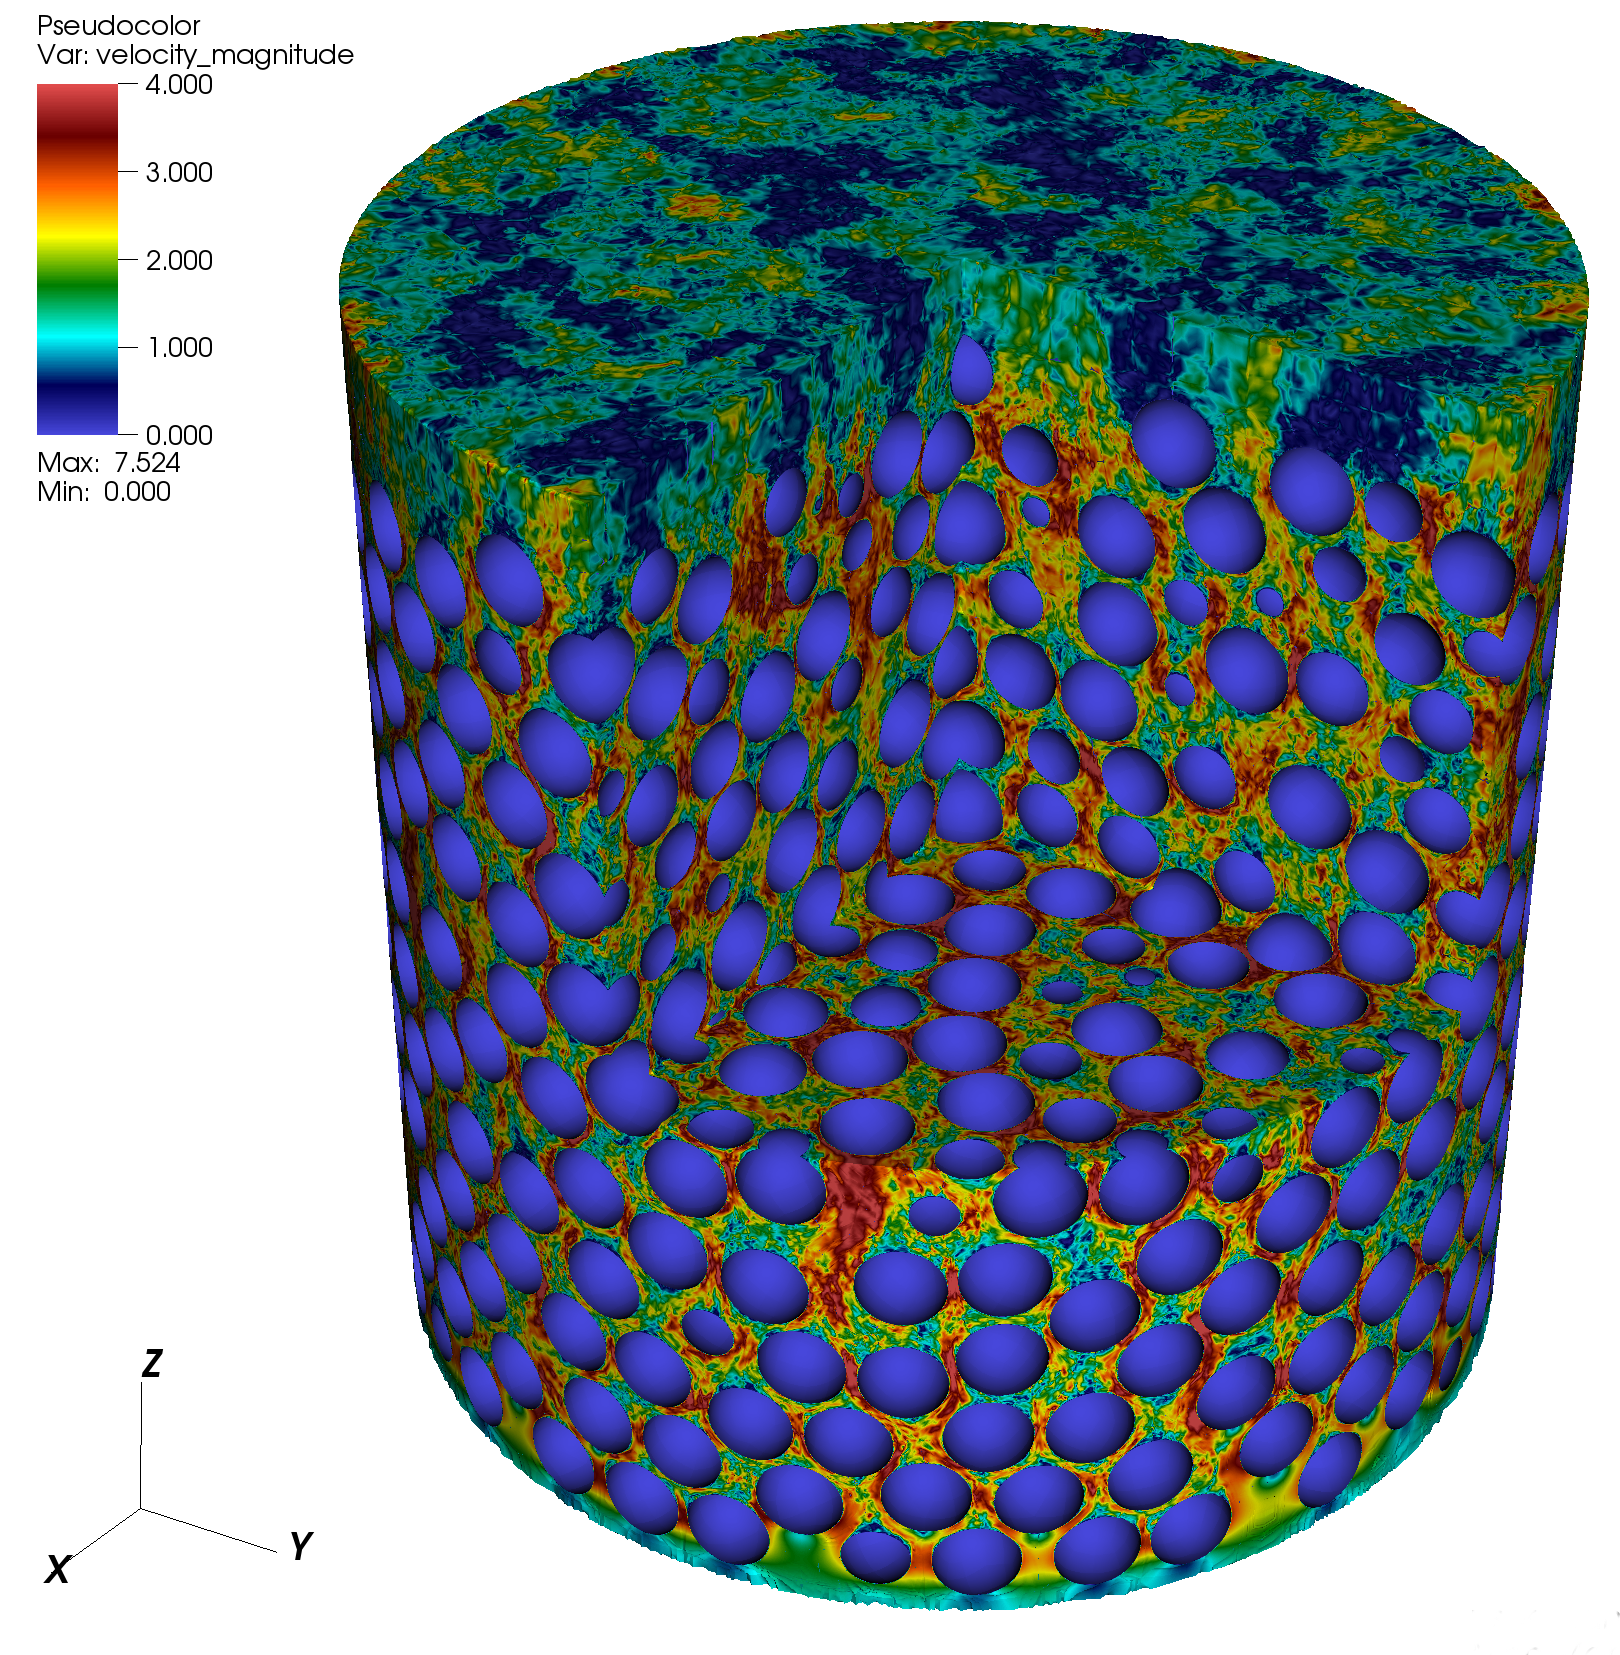
\includegraphics[clip=true,width=0.9\textwidth]{Figures/ndemo_r3}
\caption{NekRS: A velocity component for turbulent flow simulations using the spectral element mesh 
with 524,386 spectral elements for 1568 pebbles from the all-hex meshing tool based on Voronoi cell strategy. }
\label{f:ndemo3}
\end{figure}


\begin{figure}[!h]
\centering
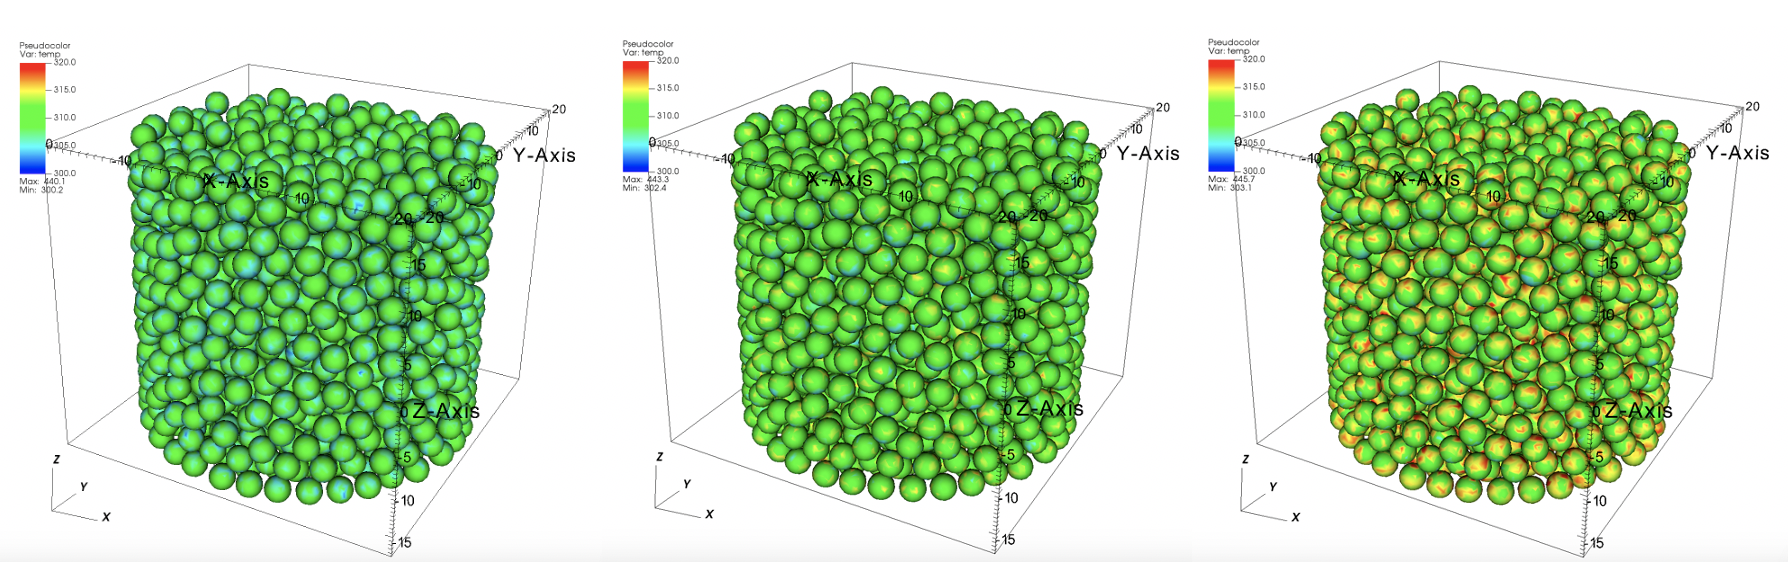
\includegraphics[clip=true,width=0.9\textwidth]{Figures/ndemo_r4}
\caption{Temperature result for the pebble surface temperature at three points in time.}
\label{f:ndemo4}
\end{figure}

The results of OpenMC simulations coupled with the heat conduction module are
shown in Figures~\ref{f:1568_openmc_heat_source} and
~\ref{f:1568_openmc_temperatures} with the same time step parameters as the
NekRS simulations described above. An eigenvalue simulation using 150 batches
with 50 inactive batches was executed in each time step. 50,000 particles per
batch were used to converge the pebble-averaged heat source from the OpenMC cell
tally while the unstructured mesh heat source tally required 500,000 particles
per batch to produce the heat source presented here. Production simulations may
require an even higher number of particles per batch to more tightly converge
the heating distribution when using the unstructured mesh heat source due to the
decreased number of samples per source particle in the tally bins.
Figure~\ref{f:1568_openmc_temperatures_single_pebble} demonstrates the effect of
the improved spatial resolution provided by the unstructured mesh heat source
from OpenMC on the temperature distribution within a representative pebble. In
the case of the pebble-averaged heat source the temperature profile is
symmetric, reflecting the uniform heat source applied in that region, while an
asymmetry can be seen in the profile generated from the unstructured mesh heat
source indicating that the improved spatial resolution of the source has an
impact on the temperature distribution in the solid and will in turn affect the
resulting heat transfer to the fluid.

\begin{figure}[!h]
\centering
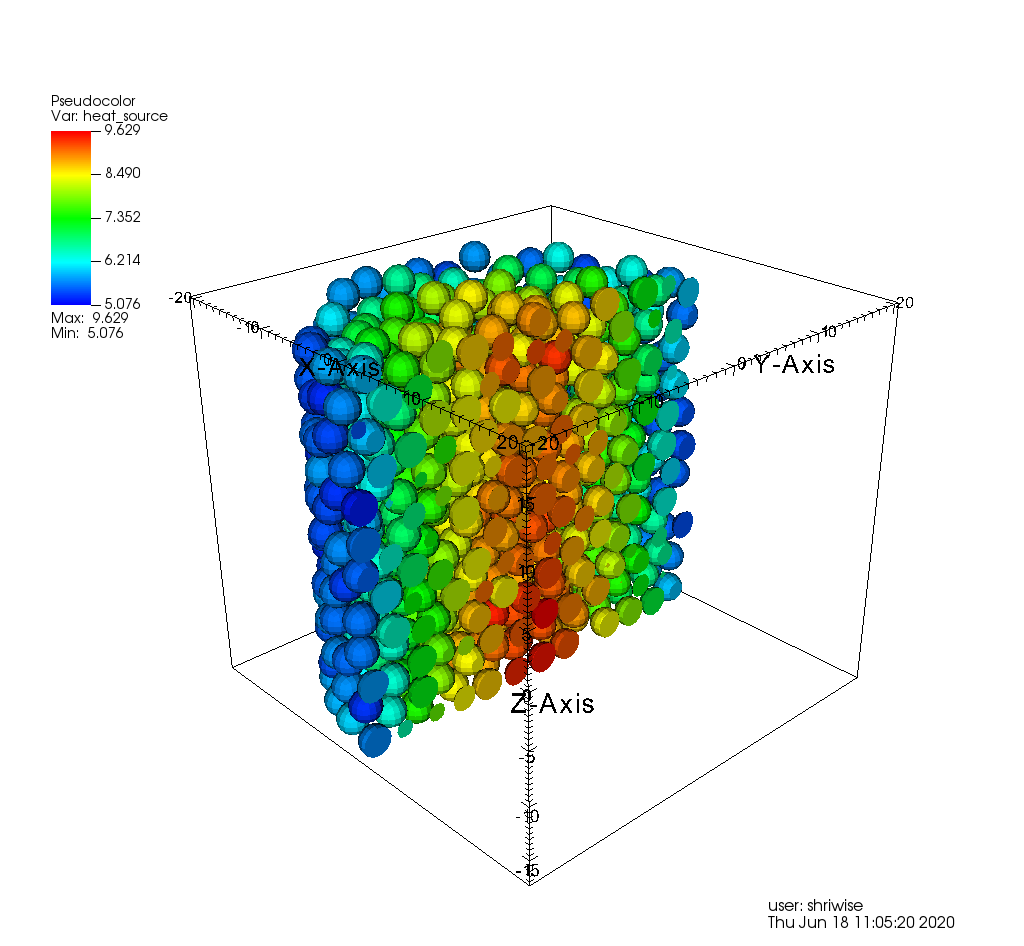
\includegraphics[clip=true,width=0.48\textwidth]{Figures/openmc_cell_heat_source}
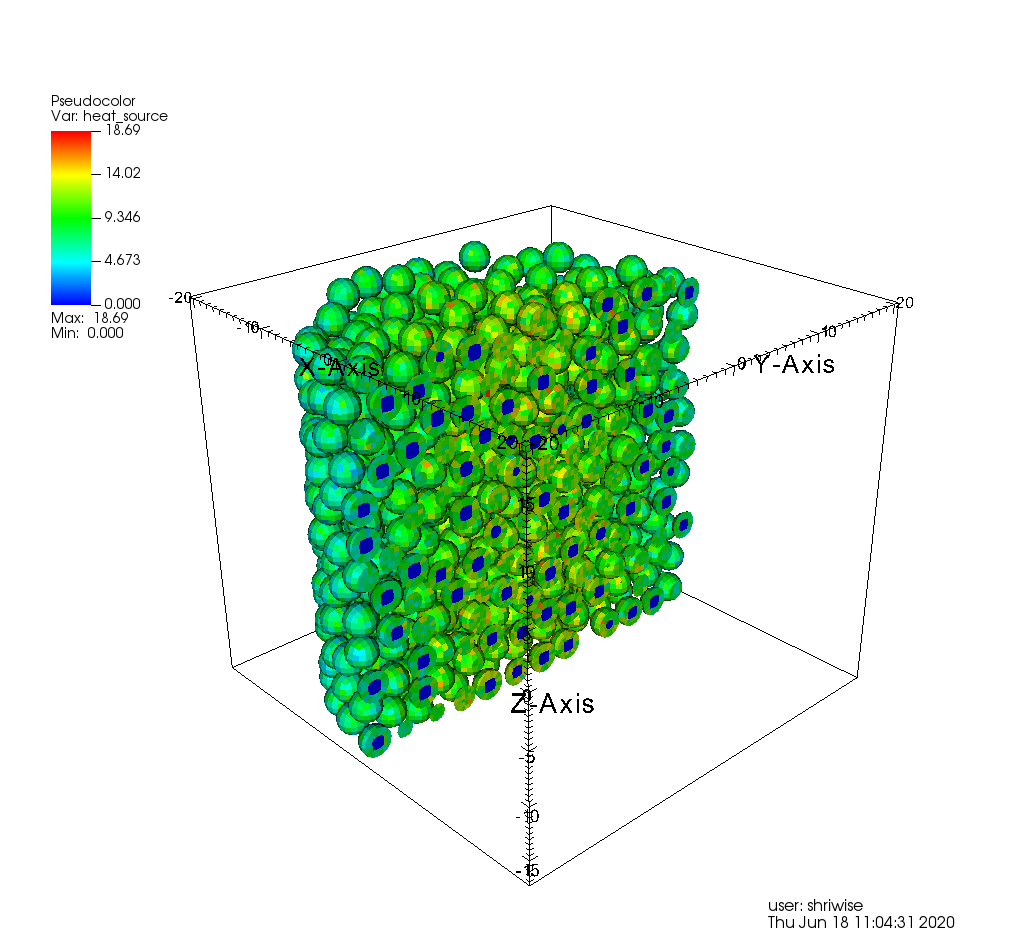
\includegraphics[clip=true,width=0.48\textwidth]{Figures/openmc_mesh_heat_source}
\caption{Left: Heat source using the original cell tallies to produces an average heat source per-pebble. Right: Heat source produced using an OpenMC unstructured mesh tally.}
\label{f:1568_openmc_heat_source}
\end{figure}

\begin{figure}[!h]
\centering
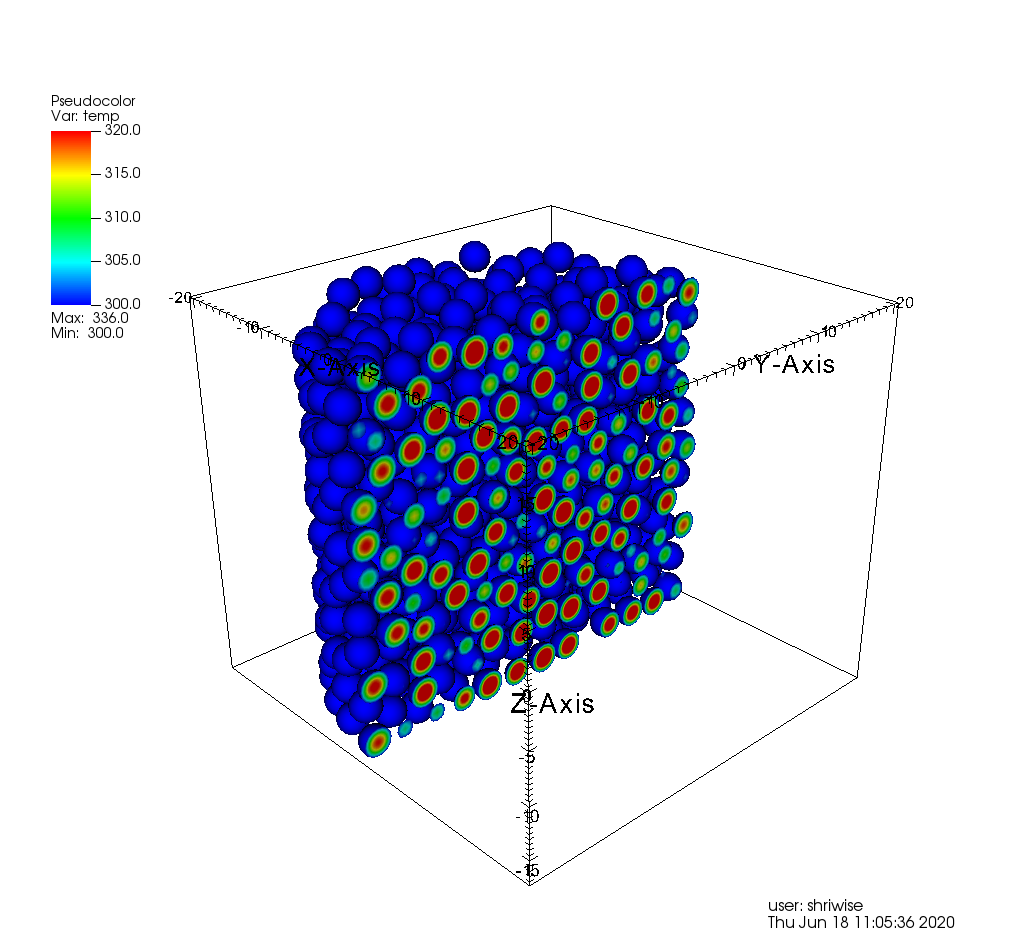
\includegraphics[clip=true,width=0.48\textwidth]{Figures/openmc_cell_temperature}
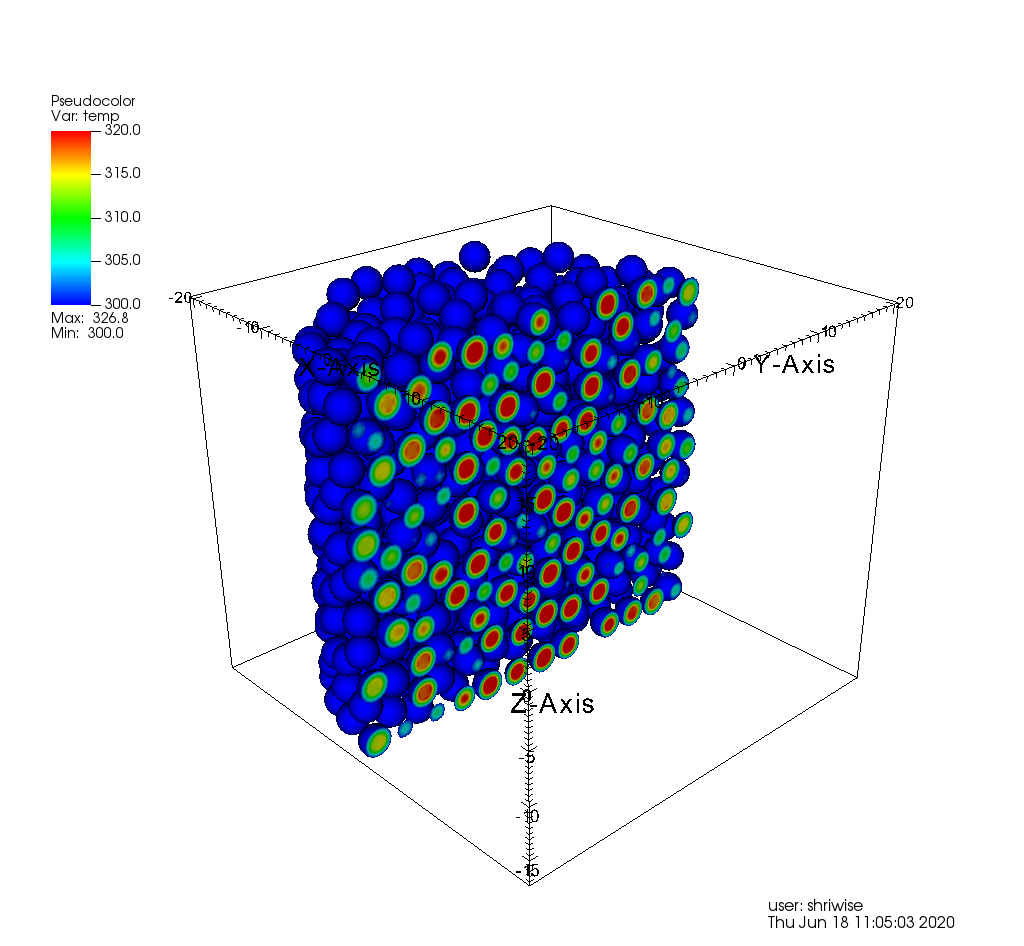
\includegraphics[clip=true,width=0.48\textwidth]{Figures/openmc_mesh_temperature}
\caption{Left: Temperature in the solid resulting from the cell-based heating tally. Right: Temperature in the solid resulting from the unstructured mesh heating tally in OpenMC.}
\label{f:1568_openmc_temperatures}
\end{figure}

\begin{figure}[!h]
\centering
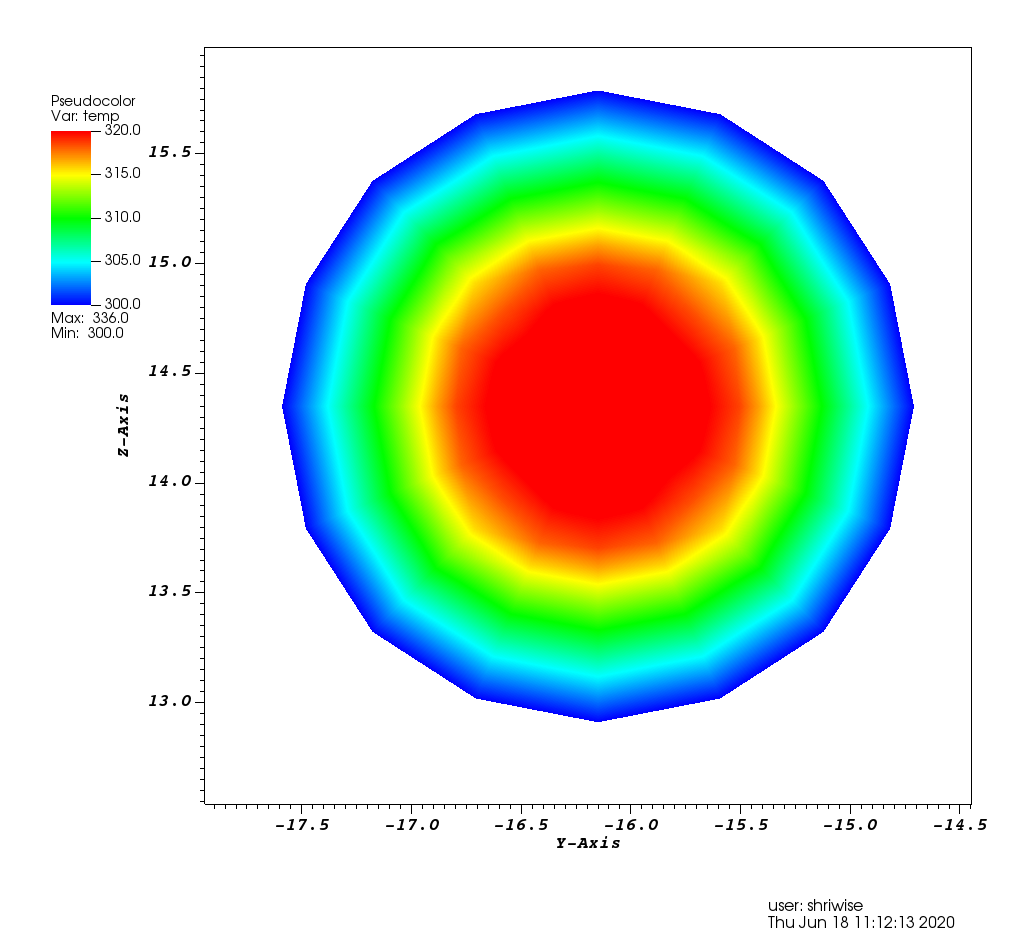
\includegraphics[clip=true,width=0.48\textwidth]{Figures/openmc_cell_temperature_zoomed}
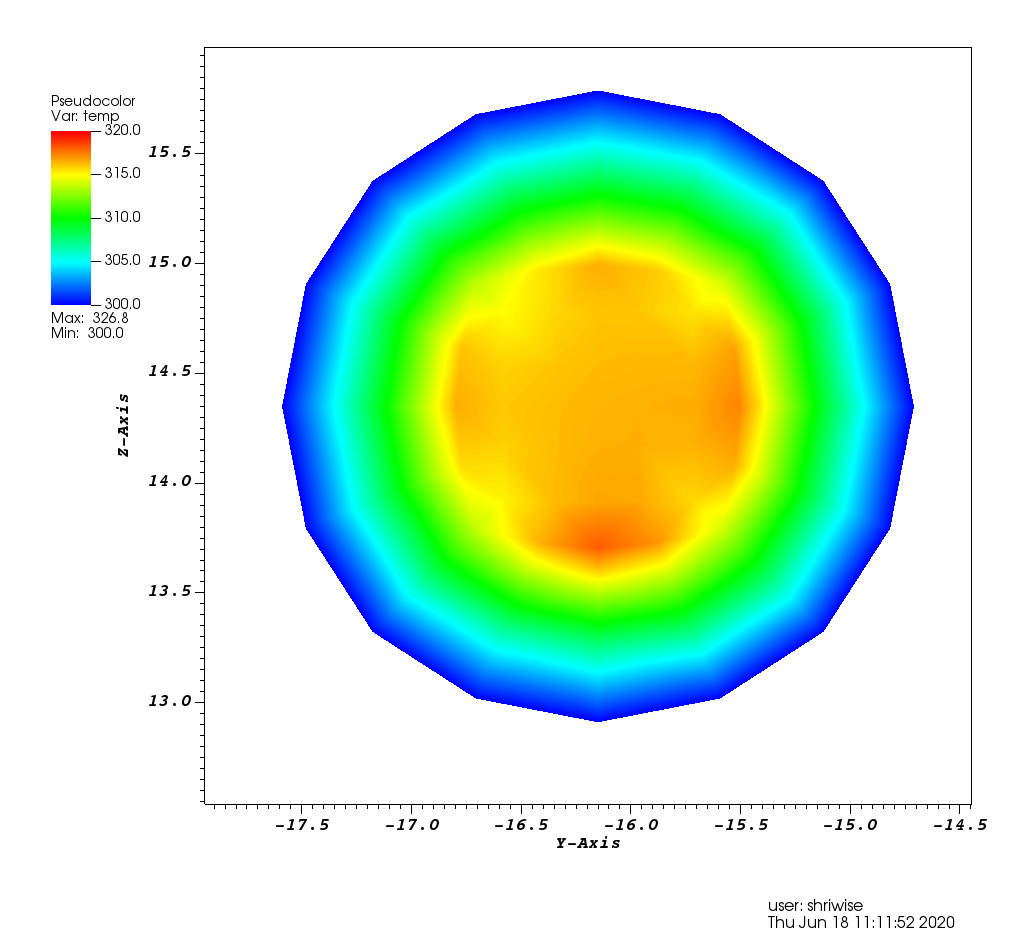
\includegraphics[clip=true,width=0.48\textwidth]{Figures/openmc_mesh_temperature_zoomed}
\caption{Temperature profiles of the same pebble in the 1568 pebble demo using the pebble-averaged heating (left) and the unstructured mesh heating (right).}
\label{f:1568_openmc_temperatures_single_pebble}
\end{figure}

\subsection{Projection to Full Core}

Twenty nodes of Summit represents less than 1\% of the computing power available on Summit. We estimate that 80\% of the machine will be sufficient to perform full core calculation in FHRs corresponding to 300,000 pebbles.
